\documentclass[11pt,a4paper]{scrartcl}
\typearea{12}
\usepackage{graphicx}
\usepackage{pstricks}
\usepackage{listings}

\usepackage{tikz}
\usepackage{amsmath}



\tikzset{
    state/.style={
           rectangle,
           rounded corners,
           draw=black, very thick,
           inner sep=2pt,
           text centered,
           },
}
\tikzset{
    on/.style={
           circle,
           draw=red, very thick,
           inner sep=2pt,
           fill=red!25,
           },
}


\tikzset{
    off/.style={
           circle,
           draw=blue, very thick,
           inner sep=2pt,
           text centered,
           },
}



\lstset{language=python}
\pagestyle{headings}
\markright{PHPH20007 - 17 computational neuroscience 1 - Conor Houghton}
\begin{document}

\section*{Introduction}

In neuroscience computational methods are used in analyzing data and
in modeling, which is what we aim to discuss here. Modeling, in turn,
is both a tool for testing out ideas about the functional significance
of an experimental discovery and a language for phrasing ideas about
brain function. This lecture is about the first of these two: modeling
as a tool for testing functional significance. The idea here is that a
neuroscience might be interested in a neuroscientific phenomenon, for
example, very fast oscillations in the hippocampus and may have
discovered a possible explanation for how the phenomenon occurs, in
the hippocampus example, axon-to-axon gap junctions. Modeling might
then be useful in seeing if the potential explanation is likely to be
correct. Gap junctions, for example, are very difficult to block, so
it might be hard to resolve this issue experimentally and so an
alternate approach would be to use a computer to try to simulate a
network of neuron with axon-to-axon gap junctions to see if the
network supports very fast oscillations. Precisely this approach is
described in \cite{TraubBibbig2000}.

The challenge then is to simulate the behavior of neurons and networks
of neurons. In fact, a lot is known about how neurons behave, but when
simulating a trade-off needs to be made between a very accurate and
detailed model which may be very slow to simulate and may contains
lots of parameters which are hard to fix using experimental data, and
very simple models that are easier to simulate and contain few
parameters, but are inaccurate and may not incorporate important
aspects of the dynamics.


\section*{Buckets of water}

In the simplest model of neurons their voltage dynamics is similar to
the dynamics of a bucket with a leak and the class of equations that
apply in this case will also be applied to synapses, for example.

\begin{center}
\setlength{\unitlength}{2mm}
\begin{picture}(20,40)
\linethickness{0.3mm}
\put(7,5){\line(1,0){8}}
\put(15,5){\line(0,1){20}}
\put(5,5){\line(0,1){20}}
\put(15,25){\line(-1,0){10}}
\put(6,5){\vector(0,-1){3}}
\put(10,27){\vector(0,-1){5}}
\put(17,10.5){\vector(0,-1){5.5}}
\put(17,14.5){\vector(0,1){5.5}}
\linethickness{0.075mm}
\put(5,20){\line(1,0){10}}
\put(7,2){$l(t)$}
\put(11,27){$i(t)$}
\put(16,12){$h(t)$}
\end{picture}
\end{center}

Consider a bucket, with straight sides which is filled to a height $h$
with water. Imagine the water leaks out of a hole in the bottom. The
rate the water leaks out depends on $h$; the larger $h$ is the larger
the pressure at the bottom is and hence the faster the water pours
out. In other words
\begin{equation}
l(t)\propto h(t)
\end{equation}
or 
\begin{equation}
l(t)= G h(t)
\end{equation}
where $G$ is a constant which will depend on the size of the hole and
complicated things like the viscosity of water. Of course, we are also
ignore lots of other complicated stuff, like turbulence and so forth, but
since we are interested in the equation rather than the amount of
water in a bucket, this is fine. Imagine water also pours in the top
at a rate $i(t)$. This means the total rate of change of the amount of
water is $i(t)-Gh(t)$.

Now, $h(t)$ is the height of the water not the volume: the volume is
$Ch(t)$ where $C$ is the cross-sectional area of the bucket. The rate
of change of the volume is therefore
\begin{equation}
\frac{dCh(t)}{dt}=i(t)-Gh(t)
\end{equation}
or
\begin{equation}
\frac{dh}{dt}=\frac{1}{C}(i-Gh)
\end{equation}
In other words, the rate that the height of the water changes is
proportional to the amount of water flowing in minus the amount
flowing out.

\subsection*{Constant input}

This equation can be solved analytically if the current flowing in is
constant, but we won't try that calculation here since it only works
for this specific special case, normally we have to solve numerically,
using a computer. The solution is
\begin{equation}
h(t)=[h(0)-i/G]e^{-t/\tau}+i/G
\end{equation}
where $\tau=C/G$. This makes sense, when $h=i/G$ then the equation
says $dh/dt=0$ so this is an equilibrium point, a value where
everything stops changing. The dynamics describe the systems as
decaying exponentially to the equilibrium.

These dynamics make good intuitive sense; the more water there is in
the bucket, the higher the pressure will be at the leak and the
quicker the water will pour out. If there is just the right about of
water the rate the water pours out the leak will precisely match the
rate it pours in, this is the equilibrium. If there is more water than
required for equilibrium it will pour out faster than the flow coming
in, if there is less, it will pour out slower. Either way, as time
passes the height of the water will reach the equilibrium. The plot in
Fig.~\ref{bucket_v} illustrates this.

\begin{figure}
\begin{center}
% GNUPLOT: LaTeX picture with Postscript
\begingroup
  \makeatletter
  \providecommand\color[2][]{%
    \GenericError{(gnuplot) \space\space\space\@spaces}{%
      Package color not loaded in conjunction with
      terminal option `colourtext'%
    }{See the gnuplot documentation for explanation.%
    }{Either use 'blacktext' in gnuplot or load the package
      color.sty in LaTeX.}%
    \renewcommand\color[2][]{}%
  }%
  \providecommand\includegraphics[2][]{%
    \GenericError{(gnuplot) \space\space\space\@spaces}{%
      Package graphicx or graphics not loaded%
    }{See the gnuplot documentation for explanation.%
    }{The gnuplot epslatex terminal needs graphicx.sty or graphics.sty.}%
    \renewcommand\includegraphics[2][]{}%
  }%
  \providecommand\rotatebox[2]{#2}%
  \@ifundefined{ifGPcolor}{%
    \newif\ifGPcolor
    \GPcolorfalse
  }{}%
  \@ifundefined{ifGPblacktext}{%
    \newif\ifGPblacktext
    \GPblacktexttrue
  }{}%
  % define a \g@addto@macro without @ in the name:
  \let\gplgaddtomacro\g@addto@macro
  % define empty templates for all commands taking text:
  \gdef\gplbacktext{}%
  \gdef\gplfronttext{}%
  \makeatother
  \ifGPblacktext
    % no textcolor at all
    \def\colorrgb#1{}%
    \def\colorgray#1{}%
  \else
    % gray or color?
    \ifGPcolor
      \def\colorrgb#1{\color[rgb]{#1}}%
      \def\colorgray#1{\color[gray]{#1}}%
      \expandafter\def\csname LTw\endcsname{\color{white}}%
      \expandafter\def\csname LTb\endcsname{\color{black}}%
      \expandafter\def\csname LTa\endcsname{\color{black}}%
      \expandafter\def\csname LT0\endcsname{\color[rgb]{1,0,0}}%
      \expandafter\def\csname LT1\endcsname{\color[rgb]{0,1,0}}%
      \expandafter\def\csname LT2\endcsname{\color[rgb]{0,0,1}}%
      \expandafter\def\csname LT3\endcsname{\color[rgb]{1,0,1}}%
      \expandafter\def\csname LT4\endcsname{\color[rgb]{0,1,1}}%
      \expandafter\def\csname LT5\endcsname{\color[rgb]{1,1,0}}%
      \expandafter\def\csname LT6\endcsname{\color[rgb]{0,0,0}}%
      \expandafter\def\csname LT7\endcsname{\color[rgb]{1,0.3,0}}%
      \expandafter\def\csname LT8\endcsname{\color[rgb]{0.5,0.5,0.5}}%
    \else
      % gray
      \def\colorrgb#1{\color{black}}%
      \def\colorgray#1{\color[gray]{#1}}%
      \expandafter\def\csname LTw\endcsname{\color{white}}%
      \expandafter\def\csname LTb\endcsname{\color{black}}%
      \expandafter\def\csname LTa\endcsname{\color{black}}%
      \expandafter\def\csname LT0\endcsname{\color{black}}%
      \expandafter\def\csname LT1\endcsname{\color{black}}%
      \expandafter\def\csname LT2\endcsname{\color{black}}%
      \expandafter\def\csname LT3\endcsname{\color{black}}%
      \expandafter\def\csname LT4\endcsname{\color{black}}%
      \expandafter\def\csname LT5\endcsname{\color{black}}%
      \expandafter\def\csname LT6\endcsname{\color{black}}%
      \expandafter\def\csname LT7\endcsname{\color{black}}%
      \expandafter\def\csname LT8\endcsname{\color{black}}%
    \fi
  \fi
  \setlength{\unitlength}{0.0500bp}%
  \begin{picture}(5040.00,3528.00)%
    \gplgaddtomacro\gplbacktext{%
      \csname LTb\endcsname%
      \put(946,704){\makebox(0,0)[r]{\strut{} 0}}%
      \put(946,1131){\makebox(0,0)[r]{\strut{} 0.5}}%
      \put(946,1557){\makebox(0,0)[r]{\strut{} 1}}%
      \put(946,1984){\makebox(0,0)[r]{\strut{} 1.5}}%
      \put(946,2410){\makebox(0,0)[r]{\strut{} 2}}%
      \put(946,2837){\makebox(0,0)[r]{\strut{} 2.5}}%
      \put(946,3263){\makebox(0,0)[r]{\strut{} 3}}%
      \put(1078,484){\makebox(0,0){\strut{} 0}}%
      \put(1672,484){\makebox(0,0){\strut{} 0.5}}%
      \put(2266,484){\makebox(0,0){\strut{} 1}}%
      \put(2861,484){\makebox(0,0){\strut{} 1.5}}%
      \put(3455,484){\makebox(0,0){\strut{} 2}}%
      \put(4049,484){\makebox(0,0){\strut{} 2.5}}%
      \put(4643,484){\makebox(0,0){\strut{} 3}}%
      \put(176,1983){\rotatebox{-270}{\makebox(0,0){\strut{}$h(t)$}}}%
      \put(2860,154){\makebox(0,0){\strut{}$t$}}%
    }%
    \gplgaddtomacro\gplfronttext{%
      \csname LTb\endcsname%
      \put(3656,3090){\makebox(0,0)[r]{\strut{}$h(0)=2$}}%
      \csname LTb\endcsname%
      \put(3656,2870){\makebox(0,0)[r]{\strut{}$h(0)=3$}}%
      \csname LTb\endcsname%
      \put(3656,2650){\makebox(0,0)[r]{\strut{}$h(0)=0$}}%
    }%
    \gplbacktext
    \put(0,0){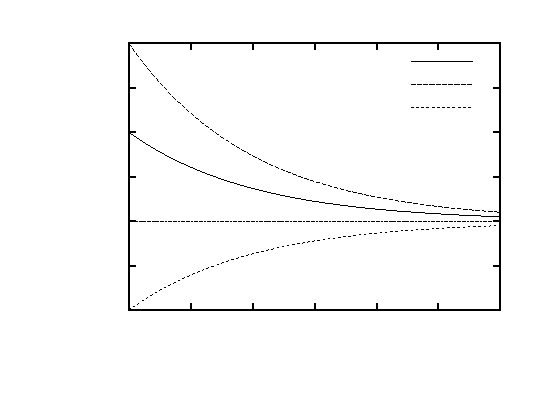
\includegraphics{bucket_v}}%
    \gplfronttext
  \end{picture}%
\endgroup

\end{center}
\caption{Exponential relaxation. The dynamics described by the
  \lq{}bucket equation\rq{} is very common. Here
  $h(t)$ is plotted with
  $i=G$, $\tau=1$ and three different values of
  $h(0)$. $h(t)$ relaxes towards the equilibrium value, the closer it gets, the slower it approaches.\label{bucket_v}}
\end{figure}

\subsection*{Variable input}

We have only discussed constant inputs; the variable input case where
$i$ depends on time is harder and although it can sometimes be solved
it is often easier just to compute it numerically, we will look
briefly at how to do this, but first note that the effect of variable
inputis that the solution kind of chases the input with a timescale
set by $\tau$, that is for very small $\tau$ is chases it quickly, so
it is close to the input, but for large $\tau$ it lags behind it and
smooths it out. This is sometimes described by saying that it
\textsl{filters} the inout. There is an illustration in
Fig.~\ref{chasing}.

\begin{figure}
\begin{center}
% GNUPLOT: LaTeX picture with Postscript
\begingroup
  \makeatletter
  \providecommand\color[2][]{%
    \GenericError{(gnuplot) \space\space\space\@spaces}{%
      Package color not loaded in conjunction with
      terminal option `colourtext'%
    }{See the gnuplot documentation for explanation.%
    }{Either use 'blacktext' in gnuplot or load the package
      color.sty in LaTeX.}%
    \renewcommand\color[2][]{}%
  }%
  \providecommand\includegraphics[2][]{%
    \GenericError{(gnuplot) \space\space\space\@spaces}{%
      Package graphicx or graphics not loaded%
    }{See the gnuplot documentation for explanation.%
    }{The gnuplot epslatex terminal needs graphicx.sty or graphics.sty.}%
    \renewcommand\includegraphics[2][]{}%
  }%
  \providecommand\rotatebox[2]{#2}%
  \@ifundefined{ifGPcolor}{%
    \newif\ifGPcolor
    \GPcolorfalse
  }{}%
  \@ifundefined{ifGPblacktext}{%
    \newif\ifGPblacktext
    \GPblacktexttrue
  }{}%
  % define a \g@addto@macro without @ in the name:
  \let\gplgaddtomacro\g@addto@macro
  % define empty templates for all commands taking text:
  \gdef\gplbacktext{}%
  \gdef\gplfronttext{}%
  \makeatother
  \ifGPblacktext
    % no textcolor at all
    \def\colorrgb#1{}%
    \def\colorgray#1{}%
  \else
    % gray or color?
    \ifGPcolor
      \def\colorrgb#1{\color[rgb]{#1}}%
      \def\colorgray#1{\color[gray]{#1}}%
      \expandafter\def\csname LTw\endcsname{\color{white}}%
      \expandafter\def\csname LTb\endcsname{\color{black}}%
      \expandafter\def\csname LTa\endcsname{\color{black}}%
      \expandafter\def\csname LT0\endcsname{\color[rgb]{1,0,0}}%
      \expandafter\def\csname LT1\endcsname{\color[rgb]{0,1,0}}%
      \expandafter\def\csname LT2\endcsname{\color[rgb]{0,0,1}}%
      \expandafter\def\csname LT3\endcsname{\color[rgb]{1,0,1}}%
      \expandafter\def\csname LT4\endcsname{\color[rgb]{0,1,1}}%
      \expandafter\def\csname LT5\endcsname{\color[rgb]{1,1,0}}%
      \expandafter\def\csname LT6\endcsname{\color[rgb]{0,0,0}}%
      \expandafter\def\csname LT7\endcsname{\color[rgb]{1,0.3,0}}%
      \expandafter\def\csname LT8\endcsname{\color[rgb]{0.5,0.5,0.5}}%
    \else
      % gray
      \def\colorrgb#1{\color{black}}%
      \def\colorgray#1{\color[gray]{#1}}%
      \expandafter\def\csname LTw\endcsname{\color{white}}%
      \expandafter\def\csname LTb\endcsname{\color{black}}%
      \expandafter\def\csname LTa\endcsname{\color{black}}%
      \expandafter\def\csname LT0\endcsname{\color{black}}%
      \expandafter\def\csname LT1\endcsname{\color{black}}%
      \expandafter\def\csname LT2\endcsname{\color{black}}%
      \expandafter\def\csname LT3\endcsname{\color{black}}%
      \expandafter\def\csname LT4\endcsname{\color{black}}%
      \expandafter\def\csname LT5\endcsname{\color{black}}%
      \expandafter\def\csname LT6\endcsname{\color{black}}%
      \expandafter\def\csname LT7\endcsname{\color{black}}%
      \expandafter\def\csname LT8\endcsname{\color{black}}%
    \fi
  \fi
  \setlength{\unitlength}{0.0500bp}%
  \begin{picture}(7200.00,5040.00)%
    \gplgaddtomacro\gplbacktext{%
      \csname LTb\endcsname%
      \put(726,440){\makebox(0,0)[r]{\strut{}-1}}%
      \put(726,873){\makebox(0,0)[r]{\strut{}-0.8}}%
      \put(726,1307){\makebox(0,0)[r]{\strut{}-0.6}}%
      \put(726,1740){\makebox(0,0)[r]{\strut{}-0.4}}%
      \put(726,2174){\makebox(0,0)[r]{\strut{}-0.2}}%
      \put(726,2608){\makebox(0,0)[r]{\strut{} 0}}%
      \put(726,3041){\makebox(0,0)[r]{\strut{} 0.2}}%
      \put(726,3475){\makebox(0,0)[r]{\strut{} 0.4}}%
      \put(726,3908){\makebox(0,0)[r]{\strut{} 0.6}}%
      \put(726,4342){\makebox(0,0)[r]{\strut{} 0.8}}%
      \put(726,4775){\makebox(0,0)[r]{\strut{} 1}}%
      \put(858,220){\makebox(0,0){\strut{} 0}}%
      \put(1453,220){\makebox(0,0){\strut{} 2}}%
      \put(2047,220){\makebox(0,0){\strut{} 4}}%
      \put(2642,220){\makebox(0,0){\strut{} 6}}%
      \put(3236,220){\makebox(0,0){\strut{} 8}}%
      \put(3831,220){\makebox(0,0){\strut{} 10}}%
      \put(4425,220){\makebox(0,0){\strut{} 12}}%
      \put(5020,220){\makebox(0,0){\strut{} 14}}%
      \put(5614,220){\makebox(0,0){\strut{} 16}}%
      \put(6209,220){\makebox(0,0){\strut{} 18}}%
      \put(6803,220){\makebox(0,0){\strut{} 20}}%
    }%
    \gplgaddtomacro\gplfronttext{%
      \csname LTb\endcsname%
      \put(5816,4602){\makebox(0,0)[r]{\strut{}$\tau=0.25$}}%
      \csname LTb\endcsname%
      \put(5816,4382){\makebox(0,0)[r]{\strut{}$\tau=2$}}%
      \csname LTb\endcsname%
      \put(5816,4162){\makebox(0,0)[r]{\strut{}$\tau=4$}}%
      \csname LTb\endcsname%
      \put(5816,3942){\makebox(0,0)[r]{\strut{}input}}%
    }%
    \gplbacktext
    \put(0,0){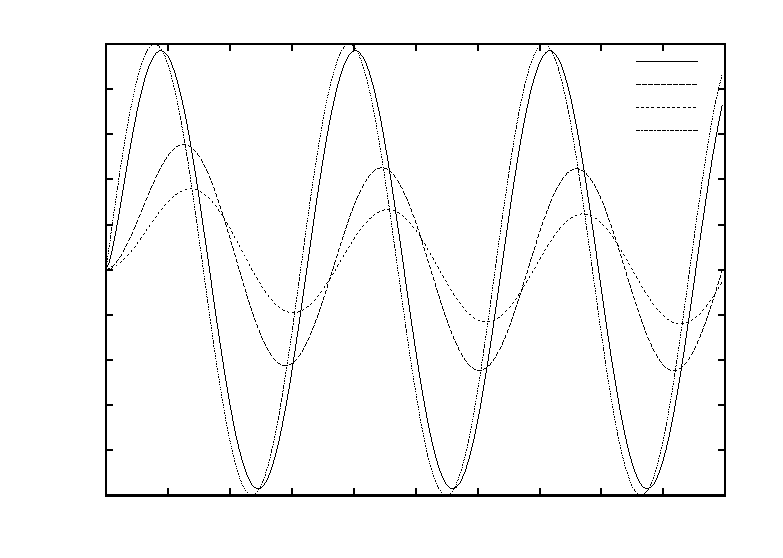
\includegraphics{chasing}}%
    \gplfronttext
  \end{picture}%
\endgroup

\end{center}
\caption{Variable input. Here the input is a sine wave $i(t)=\sin{t}$
  and the equation is evolved with $h(0)=0$ and three different $\tau$
  values. For $\tau=0.25$ we see $h(t)$ closely matches the input
  whereas for larger $\tau$ it is smoother and lags
  behind.\label{chasing}}
\end{figure}


\subsection*{Numerical solutions}

Consider the problem of solving a general first order differential equation
\begin{equation}
\frac{df(t)}{dt}=F(f,t)
\end{equation}
This includes our bucket case if we replace $f$ with $h$ and $F(f,t)$
with $(i-Gh)/C$. Now consider the situation where we want to solve
this but can't do it analytically, as will be the case for many
values of the time dependent input $i(t)$ or, indeed, if $i(t)$ itself
is only known numerically. 

The simplest numerical approach is Euler's method. Say you know the value of $f(t)$ and want to approximate $f(t+\delta t)$ where $\delta t$ is some small increment in time. Now, it is known that
\begin{equation}
f(t+\delta t)=f(t)+\delta t \frac{df(t)}{dt}+O(\delta t^2)
\end{equation}
That is, it changes by its rate of change multiplied by how long it is
changing for. The $O(\delta t^2)$ says there are $\delta t^2$ sized
errors in this approximation, this comes about because $dh/dt$ is
itself changing but our approximation assumes it is fixed still. Now we
know what $df(t)/dt$ is, it is $F(f,t)$ from the equation, so
\begin{equation}
f(t+\delta t)=f(t)+\delta t F(f,t) + O(\delta t^2)
\end{equation}
so approximating $f(t+\delta t)$ with $f(t)+\delta t F(f,t)$ is actual
to first order in the time step $\delta t$. This is the Euler
approximation. More formally if we have an initial condition $f(t_0)$ and write
\begin{align}
f_n&=f(t_0+n\delta t)\\
t_n&=t_0+n\delta t
\end{align}
then the Euler approximation is
\begin{equation}
f_{n+1}=f_n+\delta t F(f_n,t_n)
\end{equation}
Thus, in the case we are interested in here
\begin{equation}
h_{n+1}=\frac{[i(t_n)-Gh_n]\delta t}{C}
\end{equation}

Of course, this is just the easiest way to do the integration, there
are more sophisticated approaches like Runge-Kutta or backwards Euler
which are more complex and computational costly for each step, but
which are also much more accurate.

\section*{Electrical properties of a neuron}
The potential inside a neuron is lower than the potential on the
outside; this difference is created by ion pumps, small molecular
machines that use energy to pump ions across the membrane seperating
the inside and outside of the cell. One typical ion pump is
Na+/K+-ATPase (Sodium-potassium adenosine triphosphatase); this uses
energy in the form of ATP, the energy carrying molecule in the body,
and through each cycle it moves three sodium ions out of the cell and
two potassium ions into the cell. Since both sodium and potassium ions
have a charge of plus one, this leads to a net loss of one atomic
charge to the inside of the cell lowering its potential. It also
creates an excess of sodium outside the cell and an excess of
potassium inside it. We will return to these chemical imbalances
later. The potential difference across the membrane is called the
membrane potential. At rest a typical value of the membrane
potential is $E_L=-70 $mV. 

\subsection*{Spikes}

So the summary version of what happens in neuons is that synapses
cause a small increase or decrease in the voltage; excitatory synapses
cause an increase, inhibitory synapses a decrease. This drives the
internal voltage dynamics of the cell, these dynamics are what we will
learn about here. If the voltage exceeds a threshold, say $V_T=-55$ mV
there is a nonlinear cascade which produces a spike or
action potential, a spike in voltage 1-2 ms wide which rises
above 0 mV before, in the usual description, falling to a reset value
of $V_R=-65$ mV, the cell then remains unable to produce another spike
for a refractory period which may last about 5 ms. We will
examine how spikes are formed later, this involves the nonlinear
dynamics of ion channels in the membrane; first though we will
consider the integrate and fire model which ignores the details of how
spikes are produced and simplifies the voltage dynamics.

\section*{The bucket-like equation for neurons}

We will now try to extend the bucket-like equation we looked at before
so that it applies to neurons. First off we replace $h$, the height of
the water, by $V$ the voltage in the cell and $C$ will be replaced by
$C_m$, the capacitance of the membrane, the amount of electrical
charge that can be stored at the membrane is $C_mV$. The amount of
electrical charge is the analogue of the volume of water. Thus,
voltage is like height, charge is like the amount of water.

The leak is a bit more complicated, because of the chemical gradients,
that is the effects of the differing levels of ions inside and outside
the cell along and their propensity to diffuse, the voltage at which
there is no leaking of charge is not zero, it is $E_L=-70 $mV,
roughly. This is an important aspect of how neurons behave: you might
at first expect that if the voltage inside the cell was, say, -60 mV
then even if there was a high conductivity for potassium at the
membrane, the potassium ions would stay in the cell: they are positive
ions after all and so a negative voltage means the electrical force is
attracting them to the inside of the cell. However, this isn't quite
what happens, there is a high concentration of potassium inside the
cell and because of the random motion of particles associated with
temperature, these have a tendency to diffuse, that is to increase the
entropy of the situation by spreading out. It takes a force to
counteract this. This is the reversal potential, $E_L$, the voltage
required for zero current even if there is some conductivity. It turns
out that the normal Ohm's law applies around the reversal potential so
that the current out of the cell is proportional to $V-E_L$.

$G$ is now $G_m$, a conductance, measuring the porousness of the
membrane to the flow of ions, in other words, it gives the constant of proportionality for the leak current: the leak current out of the cell is
$G_m(V-E_L)$. We actually divide across by the conductance, and write
$R_m=1/G_m$, the resistance. Finally, we write $\tau_m=C_m/G_m$ to get
\begin{equation}
\tau_m\frac{dV}{dt}=E_L-V+R_mI
\end{equation}
$I$ might end up being synaptic input, but traditionally we write the
equation to match the \textsl{in vivo} experiment where $I$ is an
injected current from an electrode, so we write $I_e$, \lq{}e\rq{} for
electrode. $\tau_m$ is a time constant.

The equation above leaves out the possibility that there are other
non-linear changes in the currents through the membrane as $V$
changes. This is a problem since there are other non-linear changes in
the currents through the membrane as $V$ changes. The equation above
leaves these out, in fact, the nonlinear effects are strongest for
values of $V$ near where a spike is produced, so one approach is to
use the linear equation unless $V$ reaches a threshold value and then
add a spike \lq{}by hand\rq{}. This has the effect of changing the
voltage to a reset value, this mimics what happens in the neuron, or
in the Hodgkin Huxley model which we will look at next and which
includes the full non-linear dynamics which makes the spike. Anyway,
in summary
\begin{itemize}
\item $V$ satisfies
\begin{equation}
\tau_m\frac{dV}{dt}=E_L-V+R_mI_e
\end{equation}
\item If $V\ge V_T$ a spike is recorded and the voltage is set to a
  reset value $V_R$.
\end{itemize}
The reset value, the voltage after the spike is often set equal to the
leak potential. This is the leaky integrate and fire model, a
surprisingly old model first introduced in \cite{Lapicque1907a}. It
lacks lots of the details important in the dynamics of neurons, but is
useful and often used for modeling the behavior of large neuronal
networks or for exploring ideas about neuronal computation in a
relatively straight-forward setting.

This model is easy to solve; if $I_e$ is constant we have already
solved it above up to messing around with constants:
\begin{equation}
V(t)=E_L+R_mI_e+[V(0)-E_L-R_mI_e]e^{-t/\tau_m}
\end{equation}
If $I_e$ is not constant it may still be possible to solve the
equation, but in any case the equation can be solved numerically on a
computer. An example in given in Fig.~\ref{v_i_f}.

\begin{figure}
\begin{center}
% GNUPLOT: LaTeX picture with Postscript
\begingroup
  \makeatletter
  \providecommand\color[2][]{%
    \GenericError{(gnuplot) \space\space\space\@spaces}{%
      Package color not loaded in conjunction with
      terminal option `colourtext'%
    }{See the gnuplot documentation for explanation.%
    }{Either use 'blacktext' in gnuplot or load the package
      color.sty in LaTeX.}%
    \renewcommand\color[2][]{}%
  }%
  \providecommand\includegraphics[2][]{%
    \GenericError{(gnuplot) \space\space\space\@spaces}{%
      Package graphicx or graphics not loaded%
    }{See the gnuplot documentation for explanation.%
    }{The gnuplot epslatex terminal needs graphicx.sty or graphics.sty.}%
    \renewcommand\includegraphics[2][]{}%
  }%
  \providecommand\rotatebox[2]{#2}%
  \@ifundefined{ifGPcolor}{%
    \newif\ifGPcolor
    \GPcolorfalse
  }{}%
  \@ifundefined{ifGPblacktext}{%
    \newif\ifGPblacktext
    \GPblacktexttrue
  }{}%
  % define a \g@addto@macro without @ in the name:
  \let\gplgaddtomacro\g@addto@macro
  % define empty templates for all commands taking text:
  \gdef\gplbacktext{}%
  \gdef\gplfronttext{}%
  \makeatother
  \ifGPblacktext
    % no textcolor at all
    \def\colorrgb#1{}%
    \def\colorgray#1{}%
  \else
    % gray or color?
    \ifGPcolor
      \def\colorrgb#1{\color[rgb]{#1}}%
      \def\colorgray#1{\color[gray]{#1}}%
      \expandafter\def\csname LTw\endcsname{\color{white}}%
      \expandafter\def\csname LTb\endcsname{\color{black}}%
      \expandafter\def\csname LTa\endcsname{\color{black}}%
      \expandafter\def\csname LT0\endcsname{\color[rgb]{1,0,0}}%
      \expandafter\def\csname LT1\endcsname{\color[rgb]{0,1,0}}%
      \expandafter\def\csname LT2\endcsname{\color[rgb]{0,0,1}}%
      \expandafter\def\csname LT3\endcsname{\color[rgb]{1,0,1}}%
      \expandafter\def\csname LT4\endcsname{\color[rgb]{0,1,1}}%
      \expandafter\def\csname LT5\endcsname{\color[rgb]{1,1,0}}%
      \expandafter\def\csname LT6\endcsname{\color[rgb]{0,0,0}}%
      \expandafter\def\csname LT7\endcsname{\color[rgb]{1,0.3,0}}%
      \expandafter\def\csname LT8\endcsname{\color[rgb]{0.5,0.5,0.5}}%
    \else
      % gray
      \def\colorrgb#1{\color{black}}%
      \def\colorgray#1{\color[gray]{#1}}%
      \expandafter\def\csname LTw\endcsname{\color{white}}%
      \expandafter\def\csname LTb\endcsname{\color{black}}%
      \expandafter\def\csname LTa\endcsname{\color{black}}%
      \expandafter\def\csname LT0\endcsname{\color{black}}%
      \expandafter\def\csname LT1\endcsname{\color{black}}%
      \expandafter\def\csname LT2\endcsname{\color{black}}%
      \expandafter\def\csname LT3\endcsname{\color{black}}%
      \expandafter\def\csname LT4\endcsname{\color{black}}%
      \expandafter\def\csname LT5\endcsname{\color{black}}%
      \expandafter\def\csname LT6\endcsname{\color{black}}%
      \expandafter\def\csname LT7\endcsname{\color{black}}%
      \expandafter\def\csname LT8\endcsname{\color{black}}%
    \fi
  \fi
  \setlength{\unitlength}{0.0500bp}%
  \begin{picture}(7200.00,5040.00)%
    \gplgaddtomacro\gplbacktext{%
      \csname LTb\endcsname%
      \put(594,440){\makebox(0,0)[r]{\strut{}-70}}%
      \put(594,922){\makebox(0,0)[r]{\strut{}-60}}%
      \put(594,1403){\makebox(0,0)[r]{\strut{}-50}}%
      \put(594,1885){\makebox(0,0)[r]{\strut{}-40}}%
      \put(594,2367){\makebox(0,0)[r]{\strut{}-30}}%
      \put(594,2848){\makebox(0,0)[r]{\strut{}-20}}%
      \put(594,3330){\makebox(0,0)[r]{\strut{}-10}}%
      \put(594,3812){\makebox(0,0)[r]{\strut{} 0}}%
      \put(594,4293){\makebox(0,0)[r]{\strut{} 10}}%
      \put(594,4775){\makebox(0,0)[r]{\strut{} 20}}%
      \put(726,220){\makebox(0,0){\strut{} 0}}%
      \put(1941,220){\makebox(0,0){\strut{} 20}}%
      \put(3157,220){\makebox(0,0){\strut{} 40}}%
      \put(4372,220){\makebox(0,0){\strut{} 60}}%
      \put(5588,220){\makebox(0,0){\strut{} 80}}%
      \put(6803,220){\makebox(0,0){\strut{} 100}}%
    }%
    \gplgaddtomacro\gplfronttext{%
      \csname LTb\endcsname%
      \put(2178,4602){\makebox(0,0)[r]{\strut{} $R_mI_e=16$ mV}}%
      \csname LTb\endcsname%
      \put(2178,4382){\makebox(0,0)[r]{\strut{} $R_mI_e=12$ mV}}%
      \put(4000,0){\makebox(0,0)[r]{\strut{} $t$ (ms)}}%
      \put(0,3000){\makebox(0,0)[r]{\strut{} $V$ (mV)}}%
    }%
    \gplbacktext
    \put(0,0){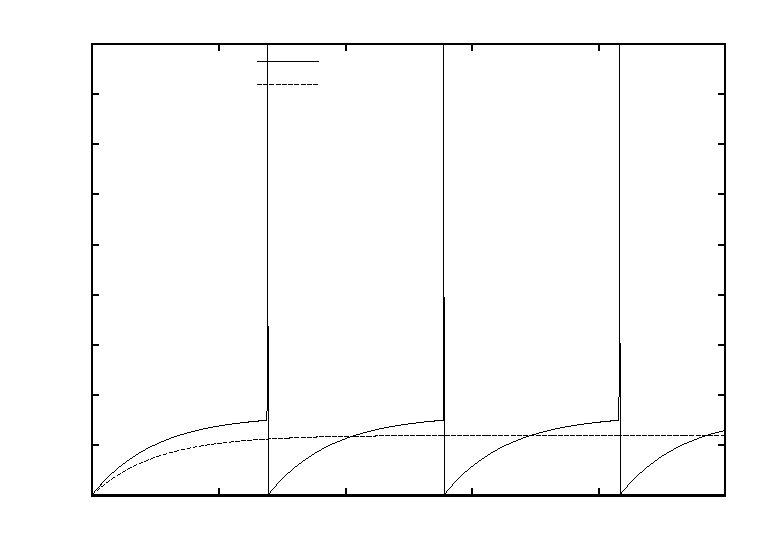
\includegraphics{v_i_f}}%
    \gplfronttext
  \end{picture}%
\endgroup

\end{center}
\caption{An integrate and fire neuron with different inputs. For
  $R_mI=12 $mV the voltage relaxes towards the equilibrium value
  $V=E_L+R_mI_e=-58$ mV. It never reaches the threshold value of
  $V_T=-55 $mV. For $R_mI=16$ mV the voltage reaches threshold and so
  there is a spike; the spike is added by hand, in this case by
  setting $V$ to $20$ mV for one time step. The voltage is then
  reset. Here $\tau_m=10$ ms.\label{v_i_f}}
\end{figure}

One thing to notice is that there are no spikes for low values of the current. Looking at the equation 
\begin{equation}
\tau_m\frac{dV}{dt}=E_L-V+R_mI_e
\end{equation}
so the equilibrium value for constant $I_e$, the value where $V$ stops changing, is
\begin{equation}
\bar{V}=E_L+R_mI_e
\end{equation}
Now if this value $\bar{V}>V_T$ then as the neuron voltage increased
towards its equilibrium value, $\bar{V}$, it would reach the
threshold, $V_T$, and spike. Hence, if $\bar{V}>V_T$ the neuron will
spike repeatedly.  However if $\bar{V}<V_T$ then the neuron will not
spike for that input because it will never reach threshold. We won't do it here\footnote{This calculation is described in \texttt{note\_on\_the\_f-I\_curve.pdf}}, but, in fact, since we can
solve the equations for constant $I_e$ we can work out the $f-I$
curve, the relationship between the firing rate and the input
current. It is plotted in Fig.~\ref{f_i_curve}.


\begin{figure}
\begin{center}
% GNUPLOT: LaTeX picture with Postscript
\begingroup
  \makeatletter
  \providecommand\color[2][]{%
    \GenericError{(gnuplot) \space\space\space\@spaces}{%
      Package color not loaded in conjunction with
      terminal option `colourtext'%
    }{See the gnuplot documentation for explanation.%
    }{Either use 'blacktext' in gnuplot or load the package
      color.sty in LaTeX.}%
    \renewcommand\color[2][]{}%
  }%
  \providecommand\includegraphics[2][]{%
    \GenericError{(gnuplot) \space\space\space\@spaces}{%
      Package graphicx or graphics not loaded%
    }{See the gnuplot documentation for explanation.%
    }{The gnuplot epslatex terminal needs graphicx.sty or graphics.sty.}%
    \renewcommand\includegraphics[2][]{}%
  }%
  \providecommand\rotatebox[2]{#2}%
  \@ifundefined{ifGPcolor}{%
    \newif\ifGPcolor
    \GPcolorfalse
  }{}%
  \@ifundefined{ifGPblacktext}{%
    \newif\ifGPblacktext
    \GPblacktexttrue
  }{}%
  % define a \g@addto@macro without @ in the name:
  \let\gplgaddtomacro\g@addto@macro
  % define empty templates for all commands taking text:
  \gdef\gplbacktext{}%
  \gdef\gplfronttext{}%
  \makeatother
  \ifGPblacktext
    % no textcolor at all
    \def\colorrgb#1{}%
    \def\colorgray#1{}%
  \else
    % gray or color?
    \ifGPcolor
      \def\colorrgb#1{\color[rgb]{#1}}%
      \def\colorgray#1{\color[gray]{#1}}%
      \expandafter\def\csname LTw\endcsname{\color{white}}%
      \expandafter\def\csname LTb\endcsname{\color{black}}%
      \expandafter\def\csname LTa\endcsname{\color{black}}%
      \expandafter\def\csname LT0\endcsname{\color[rgb]{1,0,0}}%
      \expandafter\def\csname LT1\endcsname{\color[rgb]{0,1,0}}%
      \expandafter\def\csname LT2\endcsname{\color[rgb]{0,0,1}}%
      \expandafter\def\csname LT3\endcsname{\color[rgb]{1,0,1}}%
      \expandafter\def\csname LT4\endcsname{\color[rgb]{0,1,1}}%
      \expandafter\def\csname LT5\endcsname{\color[rgb]{1,1,0}}%
      \expandafter\def\csname LT6\endcsname{\color[rgb]{0,0,0}}%
      \expandafter\def\csname LT7\endcsname{\color[rgb]{1,0.3,0}}%
      \expandafter\def\csname LT8\endcsname{\color[rgb]{0.5,0.5,0.5}}%
    \else
      % gray
      \def\colorrgb#1{\color{black}}%
      \def\colorgray#1{\color[gray]{#1}}%
      \expandafter\def\csname LTw\endcsname{\color{white}}%
      \expandafter\def\csname LTb\endcsname{\color{black}}%
      \expandafter\def\csname LTa\endcsname{\color{black}}%
      \expandafter\def\csname LT0\endcsname{\color{black}}%
      \expandafter\def\csname LT1\endcsname{\color{black}}%
      \expandafter\def\csname LT2\endcsname{\color{black}}%
      \expandafter\def\csname LT3\endcsname{\color{black}}%
      \expandafter\def\csname LT4\endcsname{\color{black}}%
      \expandafter\def\csname LT5\endcsname{\color{black}}%
      \expandafter\def\csname LT6\endcsname{\color{black}}%
      \expandafter\def\csname LT7\endcsname{\color{black}}%
      \expandafter\def\csname LT8\endcsname{\color{black}}%
    \fi
  \fi
  \setlength{\unitlength}{0.0500bp}%
  \begin{picture}(5040.00,3528.00)%
    \gplgaddtomacro\gplbacktext{%
      \csname LTb\endcsname%
      \put(814,704){\makebox(0,0)[r]{\strut{} 0}}%
      \put(814,1024){\makebox(0,0)[r]{\strut{} 10}}%
      \put(814,1344){\makebox(0,0)[r]{\strut{} 20}}%
      \put(814,1664){\makebox(0,0)[r]{\strut{} 30}}%
      \put(814,1984){\makebox(0,0)[r]{\strut{} 40}}%
      \put(814,2303){\makebox(0,0)[r]{\strut{} 50}}%
      \put(814,2623){\makebox(0,0)[r]{\strut{} 60}}%
      \put(814,2943){\makebox(0,0)[r]{\strut{} 70}}%
      \put(814,3263){\makebox(0,0)[r]{\strut{} 80}}%
      \put(946,484){\makebox(0,0){\strut{} 0}}%
      \put(1786,484){\makebox(0,0){\strut{} 5}}%
      \put(2626,484){\makebox(0,0){\strut{} 10}}%
      \put(3467,484){\makebox(0,0){\strut{} 15}}%
      \put(4307,484){\makebox(0,0){\strut{} 20}}%
      \put(176,1983){\rotatebox{-270}{\makebox(0,0){\strut{}firing rate in Hz}}}%
      \put(2794,154){\makebox(0,0){\strut{}$R_mI_e$}}%
    }%
    \gplgaddtomacro\gplfronttext{%
    }%
    \gplbacktext
    \put(0,0){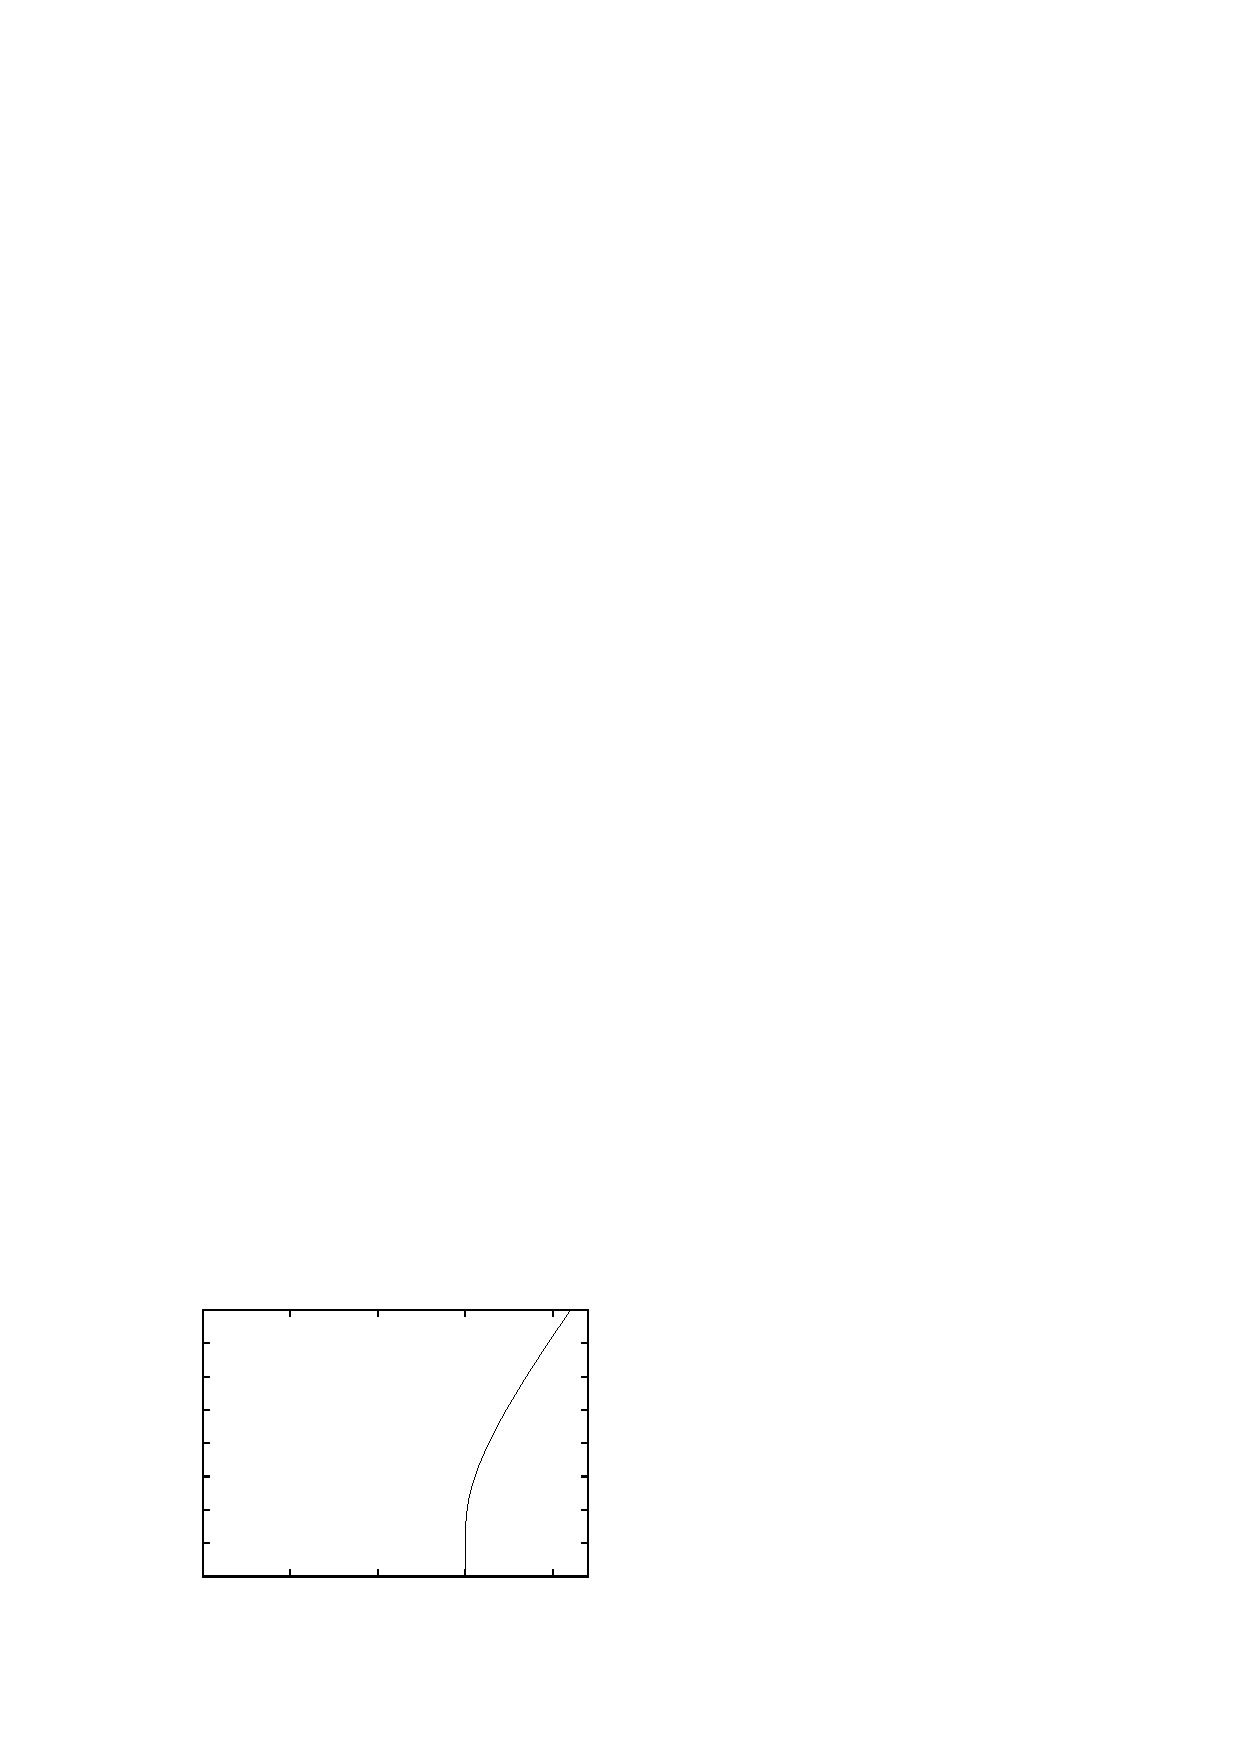
\includegraphics{f_i_curve}}%
    \gplfronttext
  \end{picture}%
\endgroup

\end{center}
\caption{The firing rate, that is spikes per second, for the integrate
  and fire neuron with different constant inputs with $\tau_m=10$ ms,
  $V_T=-55$ mV and both the leak and reset given by $-70$ mV. Notice
  how there is no firing until a threshold is reached and after that
  the firing increases very quickly. \label{f_i_curve}}
\end{figure}

\section*{The Hodgkin-Huxley equation}

The nonlinear dynamics that neurons rely on to form spikes arise from
the voltage-gated channels; these are ion channels whose
conductance varies as the voltage varies. They are, crucially, are ion
selective: only sodium ions can pass through a sodium gate, only
potassium ions through a potassium gate. This means that there are
different currents for each type of ion, whereas in the
integrate-and-fire neuron there is just the leak current, and the
conductances of these currents aren't constant, as they are for the
leak, but rather have complicated, non-linear function.  These
currents together gives the Hodgkin-Huxley equation, basically it
equates the rate of change of $V$ to a set of currents, the leak
current giving the roughly linear behavior below threshold we saw in
the integrate and fire model and the gated channels which become
important near the threshold and whose behavior gives rise to the
action potential:
\begin{equation}
C_m\frac{dV}{dt}=\mbox{currents}
\end{equation}
The currents depend on the conductances for the different ions and so
the Hodgkin-Huxley model is referred to as a conductance based model;
since the conductances depend on gated channels the equations
describing them are called gating equations.

The Hodgkin-Huxley equation has only one voltage, it pretends the
neuron is just a point. More complicated models include the spatial
extent of neurons and model the neuron as being composed of
compartments, with a Hodgkin-Huxley equation in each compartment and
what is called a cable equation describing how the compartments are
linked together.

\section*{Computational tools}

People in computational neuroscience usually use either MATLAB or
Python or they use a specialized simulation tool such as GENESIS or
NEURON or NEST. These simulation tools are optimized to efficiently
simulate large complicated neurons, in the case of GENESIS or NEURON,
or large and complicated networks of neurons, in the case of NEST. The
simulation tools have been writen over many years and can be quite
complicated and idiosyncratic, however, NEURON at least, now has a
Python interface. 

MATLAB has some advantages, it has a very large user base across many
parts of applied mathematics, a huge collection of libraries and
package. There is a free community authored version called Octave,
they are not completely compatible and Octave lacks many libraries and
features. Matlab uses a matrix paradigm which is easy to use and quick
when you get used to it. Python is a proper programming language, with
a nicer language structure than Matlab, it is free and open and has
many libraries, though perhaps not as many as Matlab.

The most specialized tools include
\begin{itemize}
\item Brian, a python package for writing neuron simulations.

\item NEURON for large biophysical simulations of neurons.

\item GENESIS, the rival to NEURON.

\item NEST, for simulating very large networks of simple neurons: http://www.nest-initiative.org/

\item XPP, a powerful tool for investigating dynamical systems of the sort found in neuroscience.

\item Open Source Brain, a set of tool for sharing neuronal simulations.

\item NeuroML, a markup language for neuron models.

\end{itemize}

\begin{thebibliography}{10}

\bibitem{TraubBibbig2000}
Traub RD, Bibbig A. (2000). A model of high-frequency ripples in the hippocampus based on synaptic coupling plus axon–axon gap junctions between pyramidal neurons. 
\newblock The Journal of Neuroscience, 20: 2086--2093.
\bibitem{Lapicque1907a}
Lapicque, L. (1907). 
\newblock Recherches quantitatives sur l'excitation électrique des nerfs traitée comme une polarisation. 
\newblock J. Physiol. Pathol. Gen, 9:620--635.

\end{thebibliography}

\end{document}
